\documentclass[a4paper, 12pt]{article}
\usepackage[T2A]{fontenc}
\usepackage[utf8]{inputenc}
\usepackage[english,russian]{babel}
\usepackage{amsmath, amsfonts, amssymb, amsthm, mathtools, misccorr, indentfirst, multirow}
\usepackage{wrapfig}
\usepackage{graphicx}
\usepackage{subfig}
\usepackage{adjustbox}
\usepackage{pgfplots}
\usepackage{wasysym}

\usepackage{geometry}
\geometry{top=20mm}
\geometry{bottom=20mm}
\geometry{left=20mm}
\geometry{right=20mm}
\newcommand{\angstrom}{\textup{\AA}}

\begin{document}
	\title{Лабораторная работа 10.1\\Электронный парамагнитный резонанс}
	\author{Нехаев Александр 654 гр.}
	\date{\today}
	\maketitle
	\tableofcontents
	\section{Введение}
	\paragraph{Цель работы} Исследовать электронный парамагнитный резонанс, определить $g$-фактор электрона, измерить ширину линии ЭПР, пронаблюдать тонкое и сверхтонкое расщепление.
	\subsection{Теоретические основы}
	Пусть ядро обладает не зависящим от внешнего поля дипольным моментом $\mu$. Взаимодействие его с полем приводит к появлению дополнительной энергии
	\begin{equation}
		E=-\mu B,
		\label{e.eq}
	\end{equation}
	где $B$ -- индукция внешнего поля. У отдельно выделенного ядра дионаправление -- направление $M$:
	\begin{equation}
		\mu=\gamma M,
		\label{mu.eq}
	\end{equation}
	$\gamma$ -- коэффициент гиромагнитного соотношения.

	Ядерный магнитон Бора:
	\begin{equation}
		\mu_{\text{я}}=\frac{e\hbar}{2m_p}=0.5\cdot 10^{-23} \text{эрг}\cdot\text{Гс}^{-2}
		\label{mu_core.eq}
	\end{equation}
	$g$-фактор:
	\begin{equation}
		g=\frac{\mu/\mu_{\text{я}}}{M/\hbar}=\frac{\mu}{\mu_{\text{я}}}\frac{\hbar}{M}=\frac{\hbar}{\mu_{\text{я}}}
		\label{g-fact.eq}
	\end{equation}
	Заменяя в (\ref{mu.eq}) $\gamma$ на $g$  с помощью (\ref{g-fact.eq}) получаем:
	\begin{equation}
		\mu=\frac{\mu_{\text{я}}}{\hbar}gM
		\label{new_mu.eq}
	\end{equation} 
	Величина $g$ изменяется не только от ядра к ядру, но и от уровня к уровню:
	\begin{equation}
		M^2=\hbar I(I+1)
		\label{m2.eq}
	\end{equation}
	где $I$ -- спиновое квантовое число (спин ядра). Проекция момента импульса квантуется:
	\begin{equation}
		M_z=m\hbar.
		\label{mz.eq}
	\end{equation}
	Из (\ref{m2.eq}) и (\ref{mz.eq}) проецируем $M$ и $\mu$ на $B$:
	\begin{equation}
		\mu_B=\frac{\mu_{\text{я}}}{\hbar}gM=\frac{\mu_{\text{я}}}{\hbar}gm\hbar=\mu_{\text{я}}gm
		\label{mub.eq}
	\end{equation}
	Различие между двумя соседними уровнями удовлетворяют условию:
	\begin{equation}
		\Delta E=B\Delta\mu_B=B\mu_{\text{я}}g\Delta m=B\mu_{\text{я}}g
		\label{deltae.eq}
	\end{equation}
	Между расщепившимися компонентами возникают переходы (с нижних на верхние) под действием высокочастотного поля. Резонансная частота определяется как:
	\begin{equation}
		\omega=\Delta E/\hbar=B\mu_{\text{я}}g/\hbar.
	\end{equation}
	Это явление называется ядерно магнитным резонансом.

	Если высокочастотное поле отсутствует, то заселенность уровней определяется по формуле Больцмана:
	\begin{equation}
		\frac{N_-}{N_+}=\exp{\left[-\Delta E/(k_{\text{Б}}T)\right]}
	\end{equation}
	где $\Delta E$ -- расстояние между уровнями. Разность заселенностей:
	\begin{equation}
		\Delta N=\Delta N_0-\left(\Delta N_0-\Delta N_1\right)\exp{\left(-t/\tau_1\right)}
	\end{equation}
	\subsection{Экспериментальная установка}
	\begin{figure}[!htb]
		\centering
		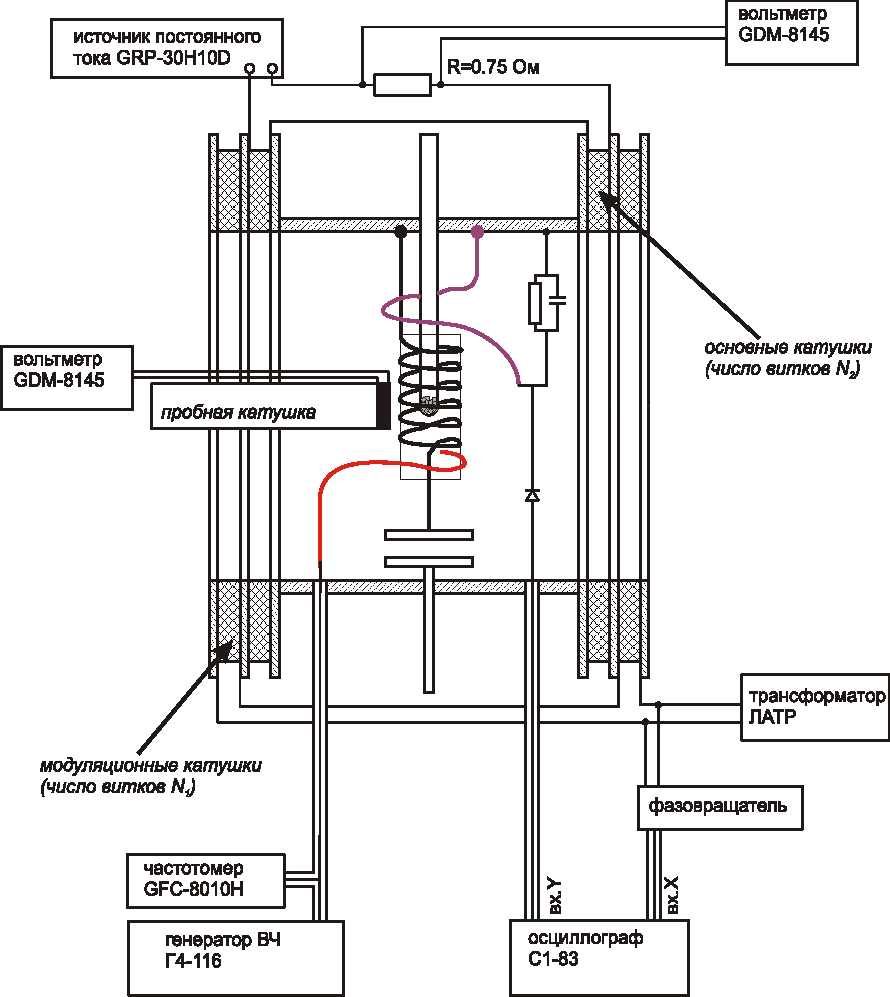
\includegraphics[scale=0.5]{scheme.pdf}
		\caption{Схема установки}
	\end{figure}
	\newpage
	\section{Ход работы}
	\subsection{Получение сигнала ЭПР  на свободном радикале ДФПГ и измерение g-фактора электрона}
	\begin{enumerate}
		\item Поместим ампулу с исследуемым веществом внутрь катушки и настроим генератор на резонансную частоту:
		\begin{equation*}
			f_{\text{res}}=128.818\text{ МГц}
		\end{equation*}
		\item Будем изменять магнитное поле в катушках таким образом, чтобы расстояние между пиками на осциллографе было одинаковым. Действующее напряжение:
		\begin{equation*}
			V=11.9\text{ мВ}
		\end{equation*}
		Параметры катушки известны: $\diameter 14.3$ мм. Следовательно $S=160.606$ мм$^{2}$. Число витков: 49. $\omega_{\sim}=2\pi*50\ Hz$. Тогда:
		\begin{equation*}
			B_0=\frac{V}{n\cdot S\cdot\omega_{\sim}}=4.81\cdot 10^{-3}\text{ Тл}
		\end{equation*}
		\item Найдем $g$-фактор электрона по полученным данным:
		\begin{equation*}
			g=\frac{\hbar\cdot\omega_0}{\mu_{\text{Б}}\cdot B}=1.91
		\end{equation*}
	\end{enumerate}
\end{document}